\section{Interface de Operação}
\label{subsec:painel_operacao}

\begin{figure*}[t]
    \centering
    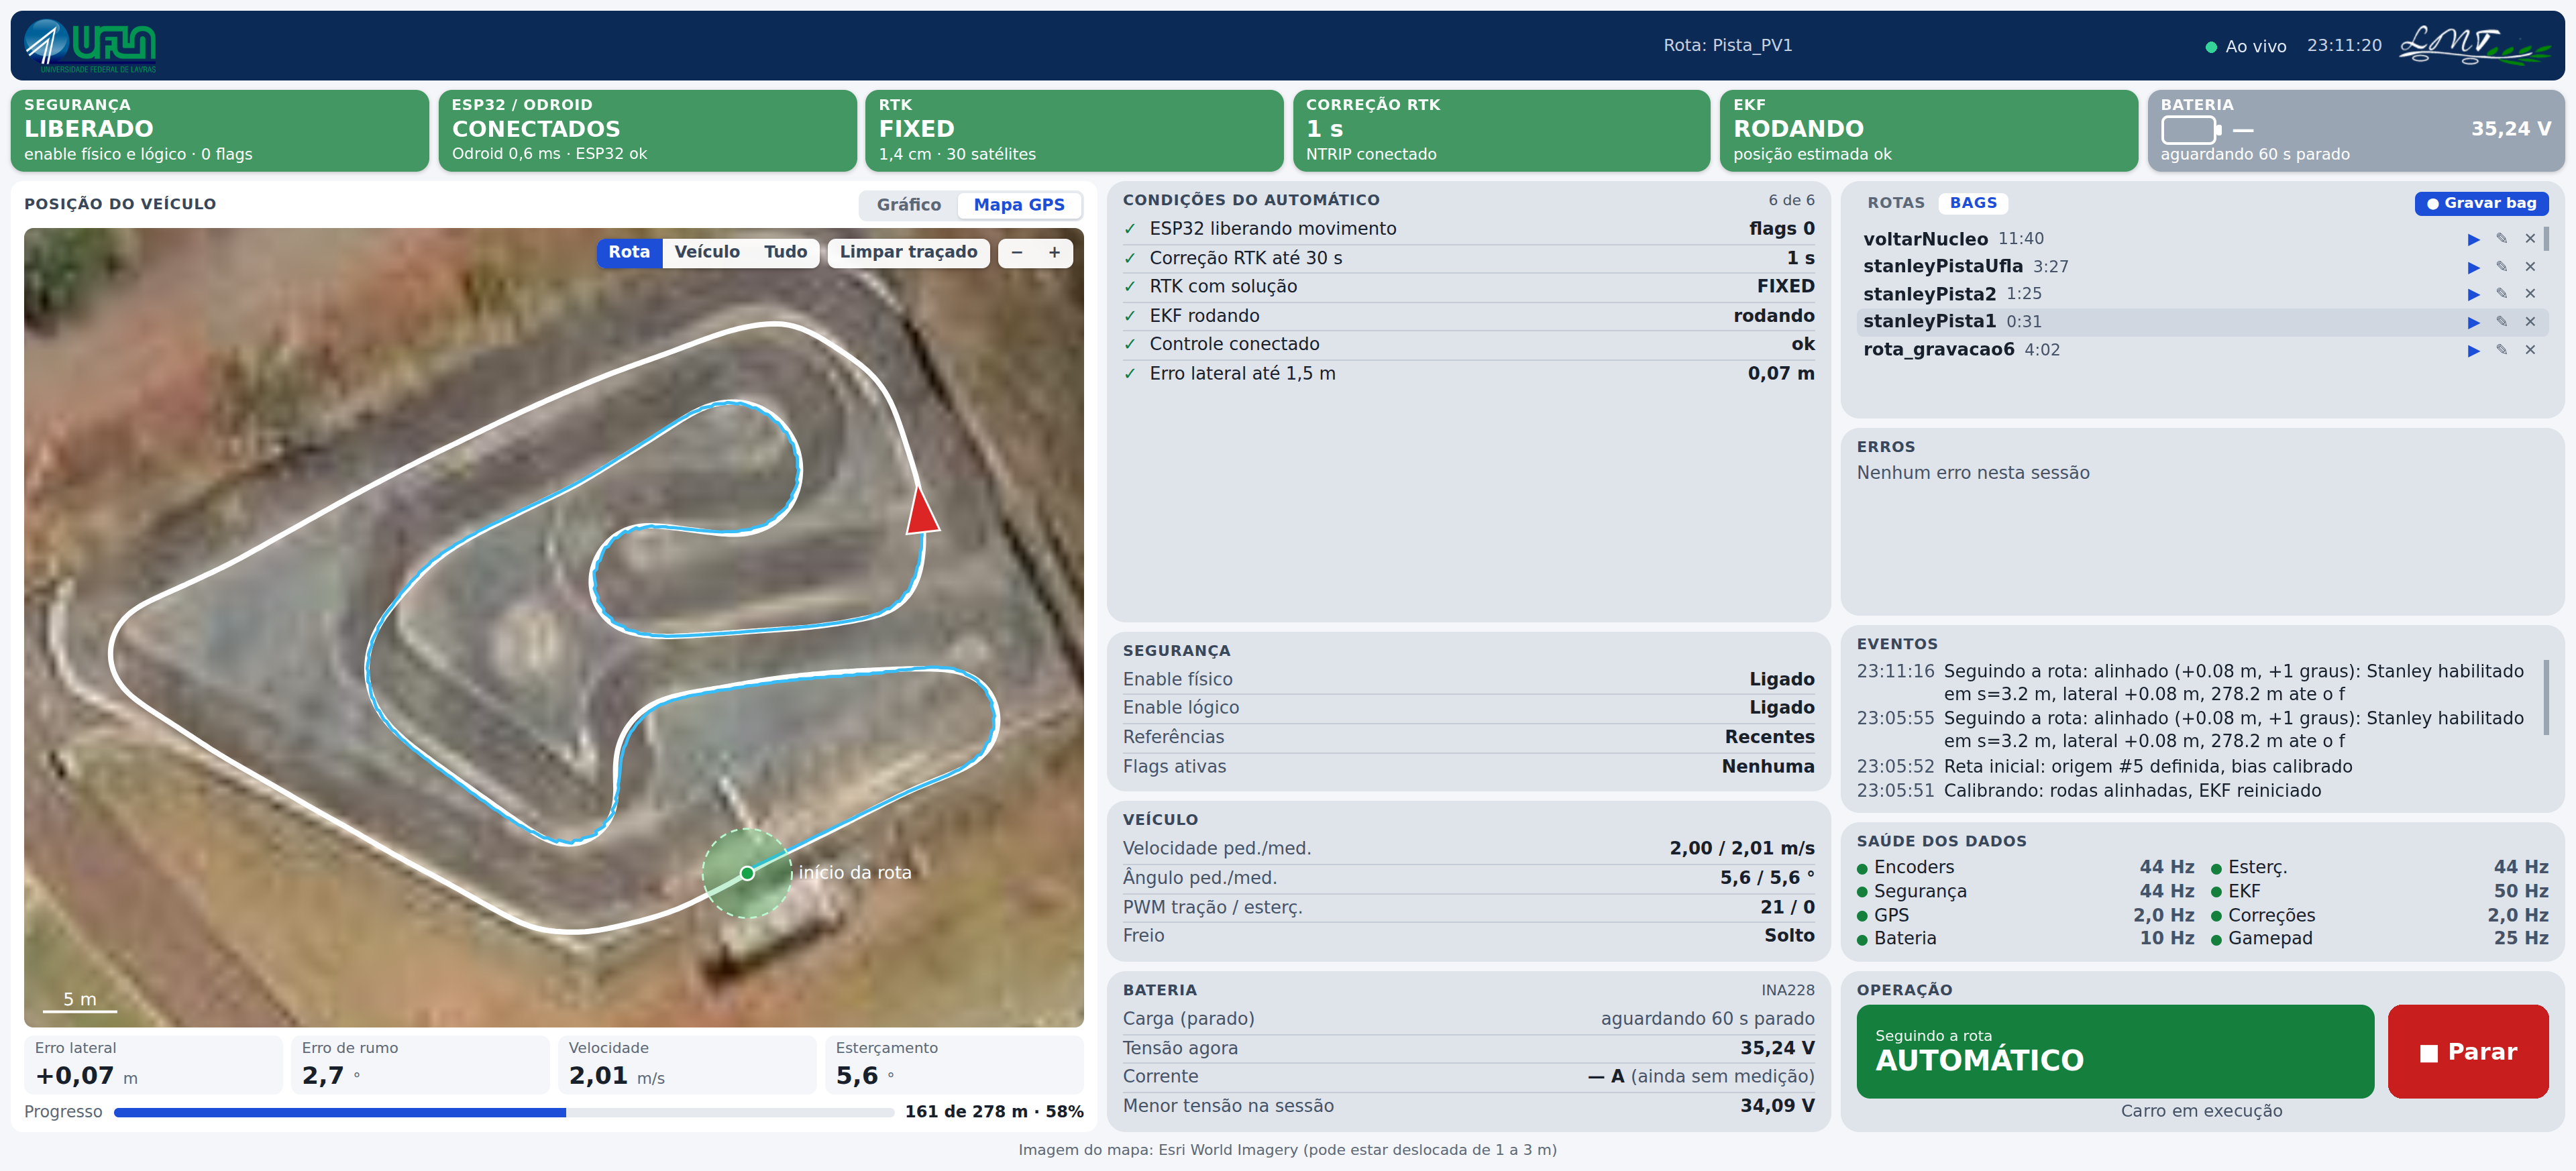
\includegraphics[width=0.98\textwidth]{Imagens/Painel_de_operacao.png}
    % legenda centralizada apenas nesta figura
    \makeatletter
    \long\def\@makecaption#1#2{\vskip 8\p@\par{\centering\@fignumfont{#1}. #2\par}}
    \makeatother
    \caption{Interface de operação e monitoramento da plataforma VIDA. Fonte: Elaborado pelo autor.}
    \label{fig:painel_operacao}
    \vspace{8pt}
\end{figure*}

Para facilitar a operação e o acompanhamento dos subsistemas da plataforma VIDA, foi desenvolvida uma interface web de supervisão, executada em um contêiner Docker no notebook de operação. O painel utiliza um servidor HTTP e  realiza atualizações periódicas via WebSocket com um nó ROS~2, que assina os tópicos de interesse e encaminha as informações à página exibida no navegador. Dessa forma, a supervisão do veículo dispensa ferramentas de visualização específicas do ROS~2 e pode ser realizada pelo próprio operador durante os ensaios.

A interface reúne, em uma única tela, informações essenciais à operação do veículo, incluindo o estado dos sistemas de segurança, condições de posicionamento GNSS/RTK, e estado do estimador de Kalman. Também permite visualizar a posição e a orientação do veículo sobre a trajetória de referência, acompanhar o progresso da navegação e consultar registros de eventos, erros e indicadores de comunicação dos subsistemas.

Além do monitoramento, o painel disponibiliza funcionalidades para iniciar e encerrar os programas de navegação, selecionar e registrar trajetórias e realizar a gravação e reprodução de dados experimentais.

A Figura~\ref{fig:painel_operacao} apresenta a interface desenvolvida, destacando a visualização da trajetória e os principais indicadores de operação e monitoramento. A centralização dessas funções em uma única interface reduz a necessidade de comandos em terminal durante os experimentos e facilita a identificação de falhas, contribuindo para a segurança e a agilidade dos ensaios.
